\chapter{Diskussion}
\label{chap_disc}


Bei der Betrachtung der Gesamtergebnisse aus den RL Experimenten, d.h. der Anzahl erfolgreich absolvierter Episoden und der dafür durchschnittlich benötigten Schrittanzahl, kann zunächst festgestellt werden, dass die Erweiterung des Schreiboperators zu einer Verbesserung der Ergebnisse führt. Darüber hinaus wirkt sich die Verwendung der GRU-basierten Schreiboperation positiv auf die Resultate aus, wenn die Aufgabenstellung schwieriger wird. Dies gilt sowohl für die Grundvariante der Neural Map als auch für die Variante mit der Erweiterung des Schreiboperators. Außerdem erzielen alle betrachteten Varianten der Neural Map bessere Ergebnisse als die Referenz, das LSTM. Da die Aufgaben in den RL Experimenten die Fähigkeiten der Modelle hinsichtlich Erkundung und Navigation überprüfen, lassen die festgestellten Verbesserungen der Resultate den Schluss zu, dass die entsprechenden Fähigkeiten durch die Verwendung des erweiterten Schreiboperators und der GRU-basierten Schreiboperation gesteigert werden. Im Rahmen des separaten Speichertests ergibt sich, dass die Neural Map und ihre Erweiterung in der Lage sind, in ihrem Speicher eine Karte der Umgebung zu generieren. Allerdings lässt sich anhand der dort verwendeten Bewertungskriterien kein Unterschied zwischen der Grundvariante und der Erweiterung festgestellen.

In Abschnitt \ref{subsec_ormg} werden in den Experimenten zwei bis vier Ziele in einem hindernisfreien Raum gesucht. Dabei werden zur detaillierten Verhaltensanalyse die Episoden in die Mengen \glqq Ziel 2/3 nie beobachtet\grqq{}, \glqq Ziel 2/3 besucht\grqq{} und \glqq Ziel 2/3 gesehen\grqq{} eingeteilt. Insbesondere die Einteilung in die zuletzt genannten beiden Mengen dient zur Untersuchung des erweiterten Schreiboperators. Für alle Mengen werden die optimale, tatsächliche und zusätzliche Schrittanzahl bestimmt. Hierbei fällt auf, dass der optimale Weg in der Menge \glqq Ziel 2/3 besucht\grqq{} für alle Größen der verwendeten Umgebung signifikant geringer ist als in den beiden anderen Mengen. Darüber hinaus enthält diese Menge im Durchschnitt erheblich weniger Episoden als die anderen beiden. Dies erscheint merkwürdig vor der Annahme, dass der Agent häufiger ein Ziel nur beobachten müsste, anstatt drüber zu laufen. Außerdem sollte der optimale Weg zwischen den Zielen für die verschiedenen Mengen näherungsweise gleich sein. Um dafür einen Erklärungsansatz zu finden, werden sich die Trajektorien diverser Episoden im Detail angeschaut. Dabei kann beobachtet werden, dass der Agent, wenn er ein Ziel beobachtet dieses in der Regel auch abläuft. Dies geschieht unabhängig davon, ob es sich um das richtige Ziel handelt oder nicht. In der kleinsten Umgebungsgröße passiert dieses Verhalten nahezu immer. Mit zunehmender Umgebungsgröße läuft der Agent auch einmal an einem Ziel, das bereits Teil seiner Observation ist vorbei. Auch dies geschieht unabhängig davon, um welches Ziel es sich handelt. Die Situation, dass er ein entsprechendes Folgeziel nur beobachtet und nicht abläuft, passiert nur, wenn er das entsprechende Folgeziel unmittelbar zusammen mit seinem eigentlich Ziel beobachtet. Die Abbildung \ref{sample_seen} enthält eine beispielhafte Trajektorie für die Menge \glqq Ziel 2 gesehen\grqq{}. Dabei sieht der Agent, wenn er sich an dem gelben Punkt befindet, innerhalb der dazugehörigen gelben Observation das Ziel 1. Dieses steuert er nun zielgerichtet an und beobachtet einen Schritt vor dessen Erreichen (entspricht dem roten Punkt) das Ziel 2. Ein Beispiel für die Menge \glqq Ziel 2 besucht\grqq{} ist in Abbildung \ref{sample_visited} dargestellt. Dabei findet der Agent bei der Erkundung zufällig Ziel 2 und läuft es dann auch entsprechend ab. Dieses Beispiel kann auch für die Menge \glqq Ziel 2 nie beobachtet\grqq{} verwendet werden, indem einfach die Positionen der beiden Ziele vertauscht werden. Ebenso kann Ziel 2 durch Ziel 3 ersetzt werden, um die entsprechenden Mengen für Ziel 3 zu verdeutlichen. Somit muss insgesamt festgestellt werden, dass die Menge \glqq Ziel 2 gesehen\grqq{} für die weitere Analyse nicht geeignet ist, da sie nur sehr spezielle Episoden enthält. Allerdings erklärt dies zumindest, warum der optimale Weg in der entsprechenden Menge deutlich kürzer ist als in den anderen Mengen.

\begin{figure}[ht!]
	\begin{subfigure}[c]{0.5\textwidth}
		%\centering
		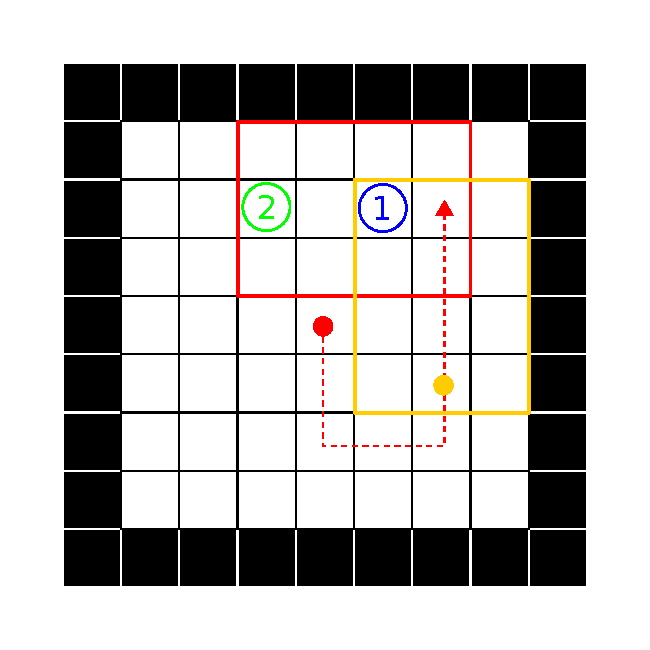
\includegraphics[keepaspectratio,width=\textwidth]{abbildungen/sample_seen.pdf}
		\subcaption{}
		\label{sample_seen}
	\end{subfigure}
	\begin{subfigure}[c]{0.5\textwidth}
		%\centering
		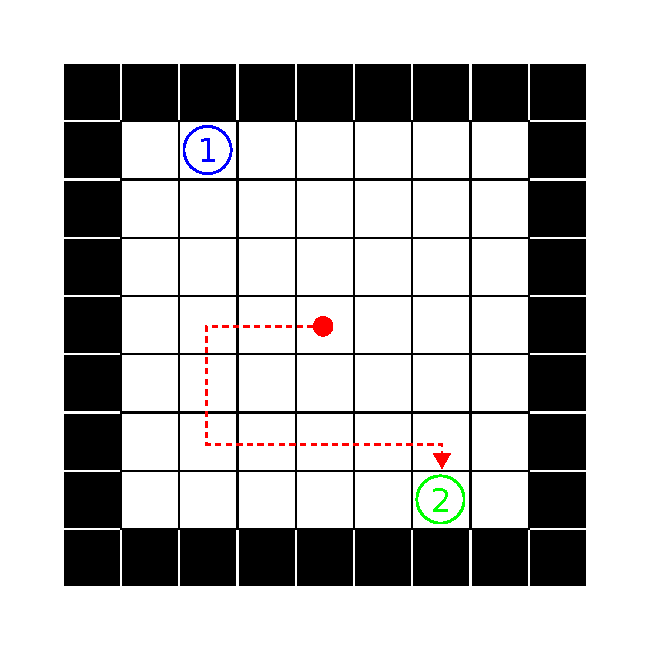
\includegraphics[keepaspectratio,width=\textwidth]{abbildungen/sample_visited.pdf}
		\subcaption{}
		\label{sample_visited}
	\end{subfigure}
	\caption{Die linke Abbildung (a) zeigt eine beispielhafte Episode für die Menge \glqq Ziel 2 gesehen\grqq{}. Für die Menge \glqq Ziel 2 besucht\grqq{} ist ein Beispiel in der rechten Abbildung (b) gegeben. Werden in diesem die Positionen der Ziele vertauscht, kann es als Beispiel für die Menge \glqq Ziel 2 nie beobachtet\grqq{} verwendet werden.}
\end{figure}

Somit werden im Folgenden nur noch die Mengen \glqq Ziel 2/3 nie beobachtet\grqq{} und \glqq Ziel 2/3 besucht\grqq{} betrachtet. Wenn der Agent in der Lage wäre, ein in der Vergangenheit bereits beobachtetes Ziel auf möglichst direktem Weg wiederzufinden, so müsste die Anzahl zusätzlicher Schritte in der Menge \glqq Ziel 2/3 gesehen\grqq{} entsprechend geringer sein. Dies ist jedoch nicht der Fall, manchmal benötigt er in der einen Menge weniger zusätzliche Schritte, manchmal in der anderen. Somit scheint er nur bedingt in der Lage zu sein, ein zuvor gesehenes Ziel gut erneut aufzusuchen. Ein Erklärungsansatz dafür könnte in der Lokalisierung des Agenten bestehen. Insbesondere in der Mitte des Raumes enthält eine Vielzahl der Observationen ausschließlich Nullen und unterscheidet sich somit nicht voneinander. Hierbei kann er die Observationen nur durch den Inhalt seiner Karte unterscheiden. Wenn er hieraus wiederum seine eigene Position nicht lokalisieren kann, ist die Information über die Lage des nächsten Ziels ebenfalls relativ wertlos. Dies erklärt ebenfalls, dass die Anzahl zusätzlicher Schritte mit zunehmender Umgebungsgröße ebenfalls stark steigt, da in diesem Fall auch die Anzahl an Observationen zunimmt, die lediglich aus Nullen bestehen. Darüber hinaus könnte auch das zuvor beschriebene Verhalten beim Zustandekommen der Mengeneinteilung finden. Die Starke Tendenz zum Ablaufen der Ziele, unabhängig davon ob es das richtige ist oder nicht, könnte ein Indiz dafür sein, dass der Agent nicht weiß, welches Ziel aktuell an der Reihe ist. Somit bringt es ihm auch nichts, die Position des Ziels in seiner Karte verzeichnet zu haben. Dieser Aspekt könnte ab drei Zielen eine Rolle spielen. In diesem Fall hat er nach dem Erreichen eines Ziels mitunter mindestens zwei Ziele zur Auswahl, die das nächste sein könnten. Da jedoch sowohl die Umgebungsgröße als auch die Anzahl der Ziele sukzessive gesteigert wird, ist es schwierig einen der beiden zuvor genannten Gründe zu favorisieren.

Des Weiteren fällt auf, dass der optimale Weg für die Menge \glqq Ziel 2/3 besucht\grqq{} immer um ungefähr einen halben bis ganzen Schritt kürzer ist im Vergleich zur Menge \glqq Ziel 2/3 nie beobachtet\grqq{}. Die Trajektorien liefern für diese Beobachtung keinen Erklärungsansatz, wodurch sie nicht erklärt werden kann.

Bei der Betrachtung der Trajektorien können jedoch noch weitere Auffälligkeiten im Verhalten des Agenten ausgemacht werden. Die Varianten mit der Erweiterung des Schreiboperators neigen stark dazu, sich zu Beginn der Episode auf der Stelle zu drehen. Dies stellt ein sehr effizientes Verhalten hinsichtlich der Erkundung dar, da auf diese Weise mit jeder Aktion die Observation maximal viele ungesehene Felder enthält. Dies ist in Abbildung \ref{sample_init_turn} veranschaulicht. Würde der Agent zu Beginn der Episode einen Schritt nach vorne gehen, so würde die daraus resultierende Observation drei unbekannte Felder enthalten (entspricht den roten Feldern). Dreht er sich jedoch auf der Stelle, so erschließt er mit der ersten Drehung acht neue Felder (blau), mit der zweiten Drehung sieben (grün) und mit der dritten Drehung sechs (gelb). Durch dieses Verhalten findet der entsprechende Agent Ziele die nah um seine Startposition liegen unabhängig von seiner initialen Blickrichtung. Es könnte sein, dass dieses Vehalten durch die Erweiterung des Schreiboperators begünstigt wird, da selbiger zumindest mit jeder Drehung auch eine neue Speicherposition beschreibt. Die Grundvarianten beschreiben bei der beschriebenen Drehung immer dieselbe Speicherstelle, da sich die Position des Agenten nicht verändert. Somit scheint die Erweiterung des Schreiboperators das Explorationsverhalten des Agenten zu verbessern. Dies wiederum stellt einen Erklärungsansatz für die insgesamt besseren Ergebnisse des erweiterten Schreiboperators dar.

\begin{figure}[ht!]
	\centering
	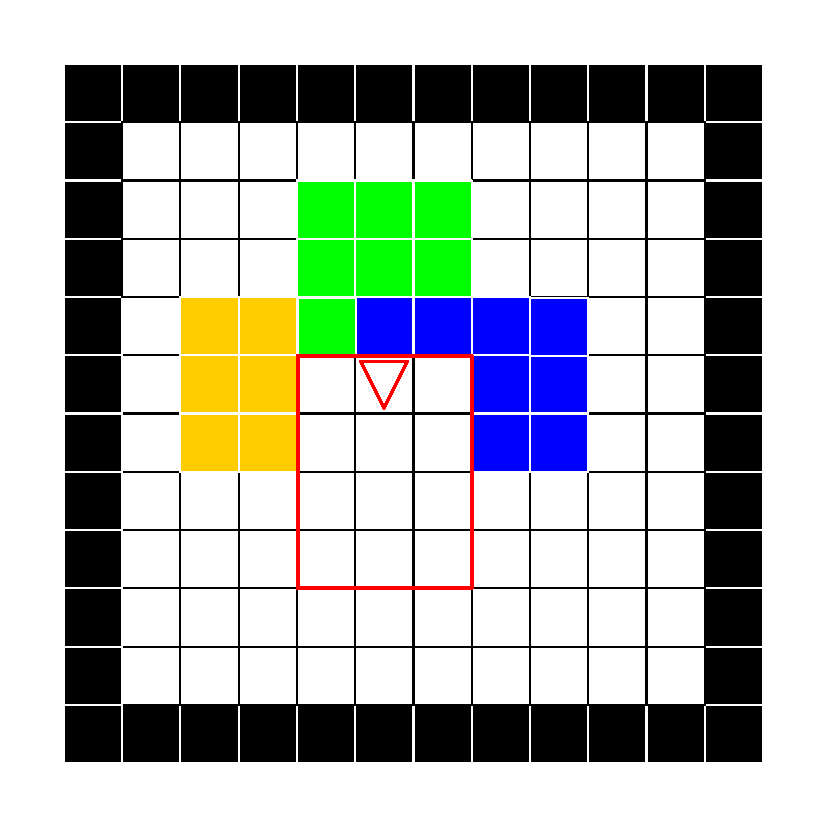
\includegraphics[keepaspectratio,width=0.5\textwidth]{abbildungen/sample_init_turn.pdf}
	\caption{Die Abbildung zeigt die neu erkundeten Felder (blau, grün, gelb), wenn der Agent sich zu Beginn der Episode zunächst auf der Stelle dreht. Zum Vergleich sind auch die neu erkundeten Felder (rot) im Falle eines Schritts nach vorne dargestellt.}
	\label{sample_init_turn}
\end{figure}

Weiterhin kann bei der Durchsicht der Trajektorien beobachtet werden, dass alle Modelle die Umgebung in Form von Kreisen erkunden. Die scheint grundsätzlich eine gute Strategie zu sein, allerdings wird dafür nicht zwingend eine Karte benötigt. Somit sind Situationen von Interesse, in denen die Modelle von diesem Muster abweichen. Dieses Verhalten kann bei den Varianten der Neural Map öfter beobachtet werden als bei dem LSTM. Insbesondere passiertfindet nach dem Erreichen eines Ziels oftmals ein Richtungswechsel bei den Neural Map Varianten statt. Allerdings kann nicht wirklich festgestellt werden, dass die Richtungsänderung zielgerichtet bezüglich des nächsten Ziels ist. Es besteht höchstens eine leichte Tendenz dazu. Darüber hinaus ist auch bei einer vermeintlich korrekten Richtungsänderung nicht gesagt, dass das nächste Ziele wirklich direkt gefunden wird.

Zur Erklärung der zuvor getätigten Beobachtungen wird zusätzlich noch ein Blick auf die Experimente im Neural Map Paper geworfen. Dabei kann festgestellt werden, dass zumindest im 2D-Experiment eine Karte der Umgebung nicht zwingend erforderlich ist. Die Aufgabe besteht im Finden eines Ziels innerhalb eines Labyrinths. Dabei gibt es zwei Ziele, wovon eines das Richtige und eines Falsche ist. Anhand eines Indikators am Anfang der Episode erfolgt die Zuteilung. Somit muss sich der Agent nur merken, welchen Indikator er gesehen hat. Der Ort an dem dies geschieht ist für die Aufgabe prinzipiell unerheblich. Allerdings bestehtmuss der Agent in einem 3D-Experiment auch zuerst ein Ziel finden und dann wieder zum Ausgangspunkt der Suche zurückkehren. Das erfolgreiche Absolvieren dieser Aufgabe, ohne auf dem Hinweg eine Karte anzulegen und diese auf dem Rückweg zu nutzen, ist nur schwer vorstellbar. Somit muss davon ausgegangen werden, dass die Neural Map grundsätzlich über diese Fähigkeiten verfügt.

Die Experimente des Abschnitts \ref{subsec_fwmg} bestehen aus der Suche von zwei bzw. drei Zielen in einem Labyrinth. Dabei ist von der Interesse inwiefern die labyrinthartige Umgebung die Zielsuche beeinflusst. Dazu werden zunächst die Ergebnisse der beiden Mengen \glqq Ziel 2/3 nie beobachtet\grqq{} und \glqq Ziel 2/3 besucht/gesehen\grqq{} analysiert. Dabei fällt auf, dass in der Menge \glqq Ziel 2/3 nie beobachtet\grqq{} grundsätzlich weniger zusätzliche Schritte benötigt werden. Erwartet wird eigentlich genau das Gegenteil. Zur Klärung werden sich auch hier wieder die Trajektorien diverser Episoden angeschaut. Es kann festgestellt werden, dass alle Modelle zu Beginn der Episode alle vier Gänge erkunden. Wird hierbei zuerst Ziel 1 gefunden (entspricht der Menge \glqq Ziel 2 nie beobachtet\grqq{}), verbleiben für die Position von Ziel 2 nur noch wahlweise zwischen einem und drei Gänge. Diese Gänge werden als nächstes erkundet, wobei dann Ziel 2 gefunden wird. Findet der Agent hingegen zuerst Ziel 2 (entspricht der Menge \glqq Ziel 2 besucht/gesehen\grqq{}), sucht er anschließend trotzdem noch alle weiteren Gänge ab unabhänig davon, in welchem er Ziel 1 findet. Erst im Anschluss daran versucht er Ziel 2 wiederzufinden. Dies erklärt die höhere zusätzliche Schrittzahl in der Menge \glqq Ziel 2 besucht/gesehen\grqq{}. Analoge Überlegungen gelten auch für Ziel 3. Bei der zuvor erwähnten initialen Erkundung der vier Gänge kann außerdem beobachtet werden, dass alle Varianten der Neural Map im Vergleich zum LSTM so gut wie nie einen Gang doppelt betreten. Dies könnte darauf hindeuten, dass die Karte der Neural Map die Exploration begünstigt.

Das Auffinden bereits gesehener Ziele fällt allen untersuchten Modellen wieder schwer. Eine Ursache dafür könnte wie in den vorherigen Experimenten sein, dass der Agent nicht weiß, welches Ziel das nächste ist. Darüber hinaus bringt das Design des Labyrinths auch noch eine für die Navigation unter Umständen ungünstige Eigenart mit. Wenn der Agent auf dem mittigen Feld steht, ist seine Observation für den linken und rechten Gang gleich. Dies könnte zu Problemen bei der Unterscheidung der beiden Gänge führen. Zur Klärung dieser Vermutung werden wieder die Trajektorien begutachtet. Dabei kann festgestellt werden, dass der Agent wirklich Probleme dabei hat ein Ziel im linken bzw. rechten Gang wiederzufinden und die Tendenz besitzt, den entsprechend anderen Gang zuerst ansteuert.

Obwohl die ursprüngliche Einteilung in drei Mengen für diese Umgebung verworfen wird, liegen die Einteilungen für drei Mengen dennoch vor. Dabei war insbesondere auffällig, dass bei drei Zielen die GRU-basierten Varianten mehrere Hundert Episoden in der Menge \glqq Ziel 2 gesehen\grqq{} haben. Es gelingt diesen Varianten somit häufiger, spätere Ziele nicht abzulaufen, sondern sich mit ihrem Anblick zu genügen. Dies kann die Anzahl benötigter Schritte reduzieren und somit eine Erklärung dafür sein, warum die entsprechenden Varianten in diesem Experiment die Ergebnisse verbessern.

Für das in Abschnitt \ref{sec_3d_exp} durchgeführte 3D-Experiment liegen lediglich Gesamtergebnisse vor, d.h. die Anzahl erfolgreicher Episoden, die durchschnittliche Schrittanzahl und der durchschnittliche Reward. Die entsprechenden Ergebnisse zeigen, dass die Erweiterung des Schreiboperators auch im wesentlich anspruchsvolleren 3D-Kontext eine Verbesserung der Neural Map darstellt. Ebenfalls wirkt sich die Verwendung des GRU-basierten Schreiboperators positiv auf die Ergebnisse aus. Somit können die Ergebnisse bzw. Erkenntnisse aus den 2D-Experimenten bestätigt werden.

Bei dem seperaten Speichertest in Abschnitt \ref{sec_mem_test} wird gezeigt, dass sowohl die Neural Map als auch ihre Erweiterung grundsätzlich die Fähigkeit besitzen, in ihrem Speicher eine Karte der Umgebung zu erzeugen. Allerdings wird dafür eine sehr hohe Anzahl an Trainingsschritten (25.000) benötigt, wenn man sie mit der maximalen Schrittanzahl in den RL Experimenten vergleicht. Dafür ist die Karte jedoch auch fehlerfrei. Ob die Neural Map eine derartig gute Karte benötigt, kann im Rahmen dieses Experiments nicht geklärt. Ebenso kann keine Verbesserung durch den Schreiboperator festgestellt werden, da dieser die gleiche Anzahl an Trainingsschritte benötigt und dabei eine Karte der gleichen Qualität liefert. Diese Aussage ist allerdings auch ein Resultat der Bewertungskriterien. Durch die Fähigkeit des erweiterten Schreiboperators auch nicht freie Felder zu beschreiben, besteht die Möglichkeit, auch Hindernisse, in diesem Fall Wände, korrekt auf der Karte zu verzeichnen. Um zu überprüfen, ob dies auch tatsächlich funktioniert, werden sich die geschätzten Umgebungsvektoren der nicht freien Felder angesehen. Dabei ergibt sich, dass die Wände korrekt abgebildet werden, d.h. der nullte Kanal enthält entsprechend eine Eins und alle anderen Kanäle eine Null. Somit kann der Karte, die von der Neural Map mit der Erweiterung des Schreiboperators erzeugt wird, eine höhere Qualität attestiert werden als der Karte der Grundvariante. Diese Aussage kann mit den ursprünglichen Bewertungskriterien nicht gewonnen werden, da diese aus Gründen der Vergleichbarkeit nur Felder berücksichtigt, die von beiden betrachteten Neural Map Varianten beschrieben werden können. Allerdings können auch nicht freie Felder wichtige Informationen über die Umgebung enthalten. So könnte beispielsweise auf einem nicht freien Feld eine verschlossene Tür sein, die sich im weiteren Verlauf noch öffnet.


\iffalse
\begin{figure}[ht!]
  %\centering
  \begin{subfigure}[c]{0.5\textwidth}
    %\centering
    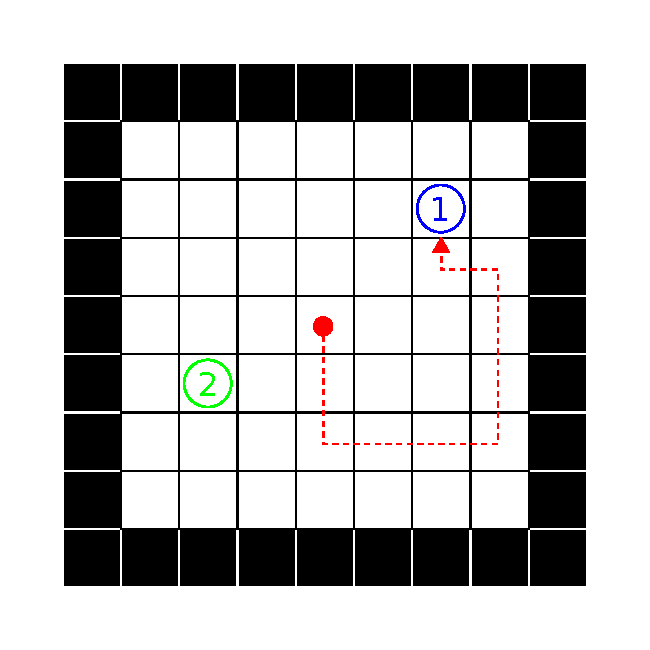
\includegraphics[keepaspectratio,width=\textwidth]{abbildungen/sample_not_seen.pdf}
    \subcaption{}
    \label{sample_visited}
  \end{subfigure}
  \begin{subfigure}[c]{0.5\textwidth}
    %\centering
    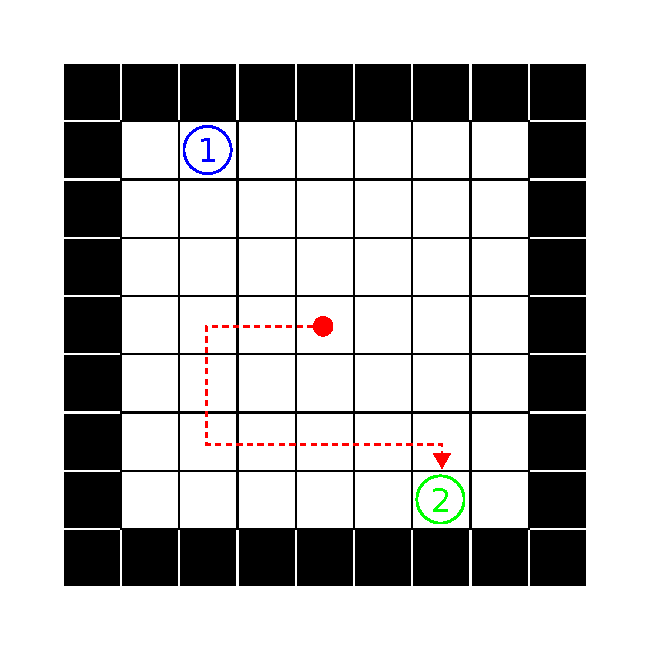
\includegraphics[keepaspectratio,width=\textwidth]{abbildungen/sample_visited.pdf}
    \subcaption{}
    \label{sample_visited}
  \end{subfigure}
  \begin{subfigure}[c]{0.5\textwidth}
    %\centering
    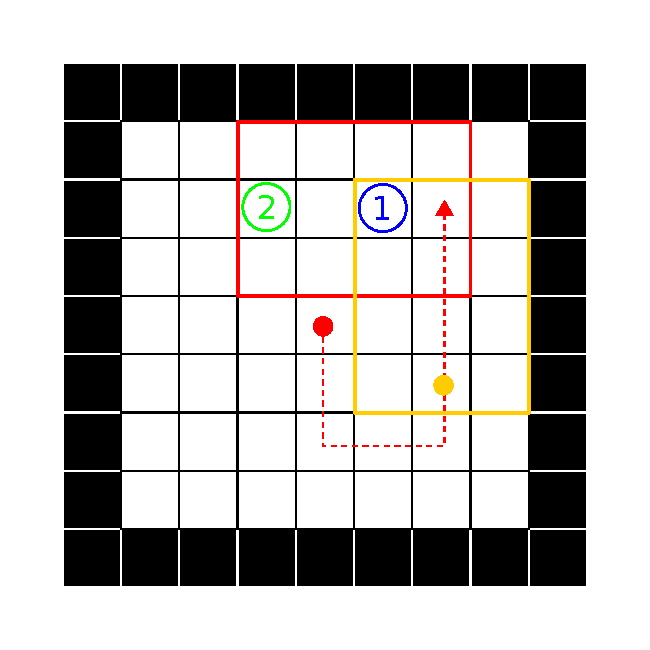
\includegraphics[keepaspectratio,width=\textwidth]{abbildungen/sample_seen.pdf}
    \subcaption{}
    \label{sample_seen2}
  \end{subfigure}
  \begin{subfigure}[c]{0.5\textwidth}
    %\centering
    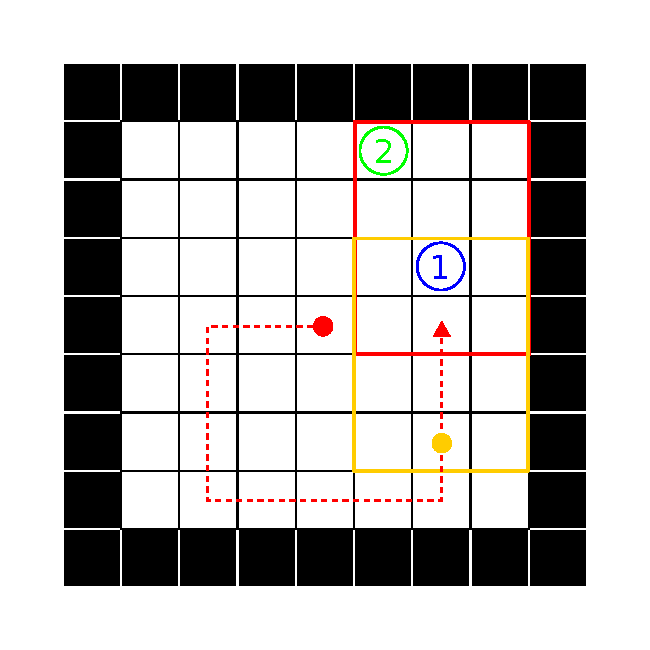
\includegraphics[keepaspectratio,width=\textwidth]{abbildungen/sample_seen2.pdf}
    \subcaption{}
    \label{sample_seen2}
  \end{subfigure}
  \caption{Blub}
\end{figure}
\fi
